\documentclass[]{article}
\usepackage{graphicx}
\usepackage{hyperref}
\usepackage{amsmath}
\usepackage{caption}
\usepackage{subcaption}
\usepackage[utf8]{inputenc}
\usepackage{float}

%opening
\title{Zeeman effect measured with a Fabry-Pérot Interferometer on the hyperfine structure of cadmium}
\author{Gunther T\"urk, Jonas Lehnen}

\begin{document}

\maketitle
\begin{abstract}
In this experiment we were able to confirm the existence of the Zeeman effect, by observing $\sigma^+$ and $\sigma^-$ polarised light of cadmiums spectral line at $643.85nm$. The measured wavelengths are very different to the expected ones, which is caused by an unknown reason.
\end{abstract}

\newpage
\tableofcontents

\newpage
\section{Introduction}
In this experiment the Zeeman effect will be discussed. In general atomic physics deals with the energy levels in an atom. With the spin orbit coupling and the fine structure, resulting from the Dirac formalism, the degeneracy of the atomic levels calculated by Bohr is lifted. Another splitting of the energy levels happens by adding another perturbation term depending on the nucleus spin. The levels of the so-called hyperfine and the fine structure are also degenerated, due to the spheric harmonics which are necessary to describe the wave function of a shell electron. This can be lifted by a static magnetic field and is called the Zeeman effect named after Pieter Zeeman in 1896.
Nowadays it is important for magnetic resonance imaging and spectroscopy of the nucleus.



\section{Theory}
\subsection{Atomic physics}
Starting with the Bohr model the energy levels are given by \autoref{eq:bohr}. The wave functions are given by a product of Laguerre and Legendre polynomials \cite{dem3}. This leads to a degeneracy of the energy levels in the n quantum number with $n^2$ levels. 

\begin{equation}
E_n = -\frac{m_ec^2\alpha^2Z^2}{2n^2} \;,\;\; \alpha=\frac{1}{137}
\label{eq:bohr}
\end{equation}

The degeneracy can be lifted by the Dirac formalism or the assumption of a perturbation by the coupling of the electrons spin $\vec{S}$ with its orbital angular momentum $\vec{L}$. The new good quantum numbers to describe the electron energy are now given by the total angular momentum $\vec{J}=\vec{L}+\vec{S}$. 
The energy shift relative to Bohr are given by \autoref{eq:energy shift fs hfs}. The same principle is applied for the hyperfine structure with $\vec{F}=\vec{J}+\vec{I}$, where  $\vec{I}$ is the nucleus spin.

\begin{align}
\Delta E_{FS}&= a\ \vec{S}\cdot\vec{L} = \frac{a}{2}\ (j(j+1)-l(l+1)-s(s+1)) \;,\quad a=  \frac{Ze^2\mu_0\hbar^2}{8\pi m_e^2r^3}\\
\Delta E_{HFS}&= b\ \vec{J}\cdot\vec{F} = \frac{b}{2}\ (f(f+1)-j(j+1)-i(i+1))\;,\quad b= \frac{g_I\mu_NB_J}{\sqrt{j(j+1)}}
\label{eq:energy shift fs hfs}
\end{align}

Where $g_s=2$ is the electrons g-factor, $g_I$ the nuclear one, $\mu_N=e\hbar/2m_P$ the nuclear magneton and $B_J$ the magnetic field induced by the electron.\\

These energy levels can then be split up another time by applying a magnetic field. The wave function can then be described by the good quantum numbers J for the fine structure, F for hyperfine, and the magnetic quantum numbers $m_j \in [-j,...,j]$, respectively $m_F$.

\newpage
\subsection{Zeeman effect}
Considering a magnetic field the magnetic moment of the electrons spin and orbital angular momentum are coupling to it and the energy levels shift apart. The example for a fine structure shift is given in \autoref{eq:Zeeman fs}. Usually the magnetic field is defined along the z-axis, therefore the eigenvalue of $j_z=m_j \hbar$ can be used.

\begin{equation}
\Delta E_{m_j} = -\vec{\mu_j}\vec{B} = \frac{\mu_B}{\hbar}(\vec{L}+g_s\vec{S})\vec{B} = \mu_B g_j m_j B 
\label{eq:Zeeman fs}
\end{equation}

The g-factor $g_j$ can be derived by the assumption of describing the energy only with $j$ and $m_j$ as good quantum numbers. This is shown in \autoref{eq:get mj}. The solution follows by multiplying with $\vec{J}$ and inserting the definition of $\vec{J}$ and the eigenvalues.

\begin{equation}
(\vec{L}+g_s\vec{S})\vec{B}  \overset{!}{=}  \vec{J}\vec{B} \;\rightarrow\; g_j = 1+\frac{j(j+1)+s(s+1)-l(l+1)}{2j(j+1)}
\label{eq:get mj}
\end{equation}

The normal Zeeman effect is for $s=0$. In this case $\vec{L}=\vec{J}$ and thereby $g_j=1$. Later in the analysis this case will be assumed.

For stronger magnetic field, the $j$ quantum numbers are no longer good. In this Paschen-Back regime the spin orbit coupling will be weaker than the energy shift by the magnetic field. Therefore $s$ and $l$ are still good and the energy shift is given by 

\begin{equation}
\Delta E_{PB}= \frac{\mu_B}{\hbar} (L_z + g_sS_z)B=\mu_B (m_l + 2m_s)B
\label{eq:paschen back}
\end{equation}


\subsection{Fabry-Pérot Interferometer}
The Fabry-Pérot Interferometer (FPI) is used to interfere light with itself. \autoref{fig:fpi} shows the general set-up. The main part are the two partial silvered mirrors in a distance d to each other, where the light gets scattered between. Due to a reflectance of $R=0.99$ in this experiment, only a fraction of the light can leave by mirror II which acts now similarly to a diffraction grating. The lens is important to let those light rays interfere with each other in a measurable distance. 

The displayed beam path difference after one cycle between the mirrors is given by \autoref{eq: path diff}. The first equation is given by shifting the path $\overline{CD}$ to the half of $\overline{AD}$ and mirroring this. For constructive interference this has to be a multiple of the wavelength.

\begin{equation}
\Delta= \overline{ABC} - \overline{AD} = \overline{A'BC'} = 2d\cdot cos(\alpha) \overset{!}{=} m\cdot \lambda
\label{eq: path diff}
\end{equation}

The position of the maximum $r_m$, depending on the order m, whereas the 0. order is infinitely far away due to $cos(90^\circ)=0$, is given in \autoref{eq:r_m}.

\begin{equation}
r_m=tan(\alpha)\cdot f\approx \alpha\cdot f
\label{eq:r_m}
\end{equation}

\begin{figure}[H]
\centering
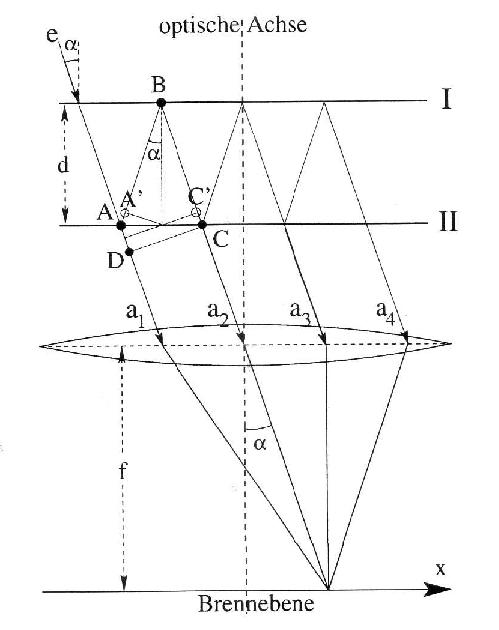
\includegraphics[width=.5\textwidth]{Plots/FPI.jpg}
\caption{Schematics of the Fabry-Pérot Interferometer. The reflective mirrors are in a distance $d$ to each other. While the lights enters in the relative angle $\alpha$ perpendicular to the mirrors. }
\label{fig:fpi}
\end{figure}

\begin{equation}
cos(\alpha) \approx 1 - \frac{1}{2}\alpha^2 \;\rightarrow\; \alpha^2 =2 - \frac{m\lambda}{d}
\label{eq:cos taylor}
\end{equation}

Combining the square of \autoref{eq:r_m} with the Taylor series of cosine for small angles, see \autoref{eq:cos taylor}, results in \autoref{eq:r_m square}.

\begin{equation}
r_m^2 = 2 f^2 - \frac{\lambda}{d}f^2\cdot m
\label{eq:r_m square}
\end{equation}

Instead of counting from the outside towards the center, we define $p$ as the order of a maximum relative to $m_0$, which is in the center of the interference muster. This results in \autoref{eq:lambda fit func} and this will be the used function to determine the wavelength, due to the definition of $m_{fit}$.

\begin{equation}
r_p^2= \left[ 2 f^2 - \frac{\lambda}{d} f^2 (m_0+1) \right] + \frac{\lambda}{d} f^2 \cdot p =: b_{fit} + m_{fit}\cdot p
\label{eq:lambda fit func}
\end{equation}

The resolving capacity of a FPI is defined as the quotient of the observed lights wavelength $\lambda_0$ and the difference between two neighbouring maxima $\delta \lambda$. The best possible value is given by \autoref{eq:resolving cap}.

\begin{equation}
\left(\frac{\lambda_0}{\delta\lambda}\right)_{FPI} = \frac{d\pi}{\lambda_0}\frac{2\sqrt{R}}{1-R}
\label{eq:resolving cap}
\end{equation}



\newpage
\section{Experimental Set-up}
\begin{figure}[H]1
\centering
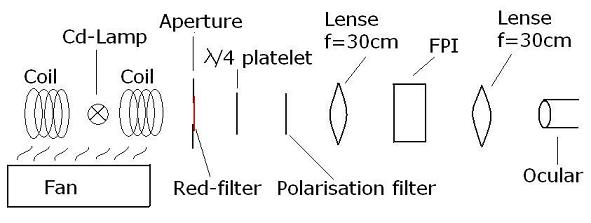
\includegraphics[width=1\textwidth]{Plots/SetupZeeman.jpg}
\caption{Set-up for measuring the Zeeman shift. For the calibration of the wavelengths, the wave plate and the polarisation filter are not used.}
\label{fig:setup}
\end{figure}

The general set-up is shown in \autoref{fig:setup}. Two coils are producing the static magnetic field, depending on the current supplies by a constant-current generator, which is not shown in the picture. The current used in this experiment is up to $50 A$, see \autoref{fig:hyst}. The magnetic field will be measured by a portable Hall effect sensor. A fan prevents the lamp and coils form melting.

In between the coils the lamps will be placed. For the Zeeman effect the cadmium lamp is used, but we'll also determine the wavelength of the red spectral line of zinc. Thereby red-filter discards all the other spectral lines given from the lamps.

The Zeeman effect will be observed on the transitions with $\sigma^+$ and $\sigma^-$ polarised light. Therefore we have to filter those polarisation with the $\lambda/4$ wave plate and the polarisation filter. The first lens focuses the light to create this relative angle to the mirror while entering the FPI, as shown in \autoref{fig:fpi}. Ocular is then placed in the focal plane of the second lens and there the interference pattern is recorded by a camera. A needle inside the ocular will be used to determine the distance between the maxima. By changing the position of the ocular in an $90^\circ$ degree angle to the entering light, the needles position will change and we can get the relative position of a maximum $r_p$.



\newpage
\section{Analysis}
\subsection{Hysteresis of magnetic field}
It is possible that while decreasing the current through the coils, the magnetic field is much stronger than for increasing current. This is called hysteresis and is caused by the magnetisation of the material. Because the magnetisation was stronger before lowering the current it is possible that the material will preserve a bit of its magnetisation.

If the difference between both directions is to grave, this has to be considered for the determination of a magnetic field for measured current. The used fit function is a polynomial of third degree given by \autoref{eq:B fit}. The current is thereby represented by the variable x.

\begin{equation}
B(x) = a\cdot x^3 + b\cdot x^2 + c\cdot x + d
\label{eq:B fit}
\end{equation}

\begin{figure}[H]
\centering
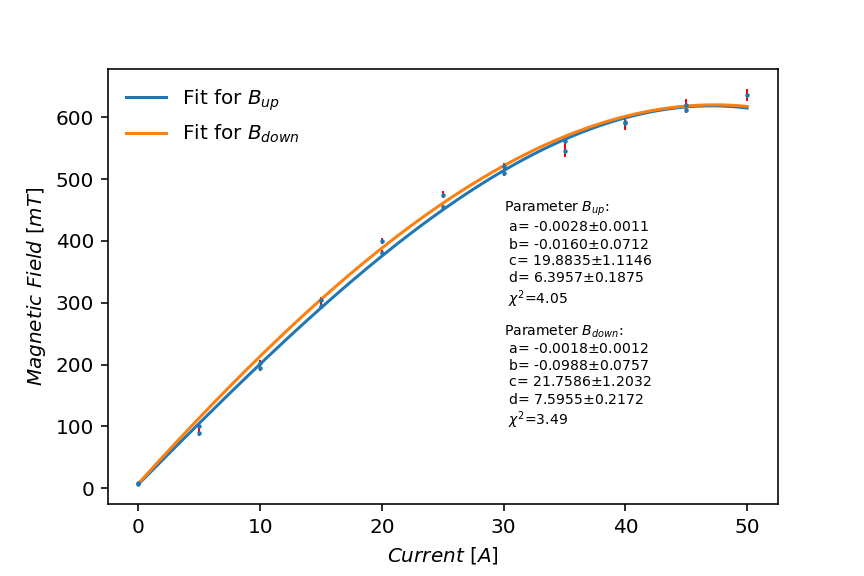
\includegraphics[width=.8\textwidth]{Plots/hysteresis.png}
\caption{Hysteresis curve for the magnetic field between both coils. The position where the lamps will be in the next chapters. Large $\chi^2$ values due to the scale of $[mT]$ and therefore large values itself. }
\label{fig:hyst}
\end{figure}

As shown in \autoref{fig:hyst} there is a difference between increasing and decreasing the current and thereby the magnetic field. As expected the values for $B_{down}$ are slightly higher than $B_{up}$. Up and Down are representing the direction of the change in current.

In the following chapters hysteresis won't be considered any longer, due to the insufficient discrepancy of the magnetic fields. The error on the magnetic field is calculated by \autoref{eq: B error}.

\begin{equation}
\Delta B(x) =  (3a\cdot x^2 + 2b\cdot x + c )\cdot \Delta x 
\label{eq: B error}
\end{equation}


\subsection{Determination of the wavelength}
By measuring the displacement of the ocular and the relative orders of the maxima \autoref{fig: lambda cd zn } was created.

\begin{figure}[H]
\centering
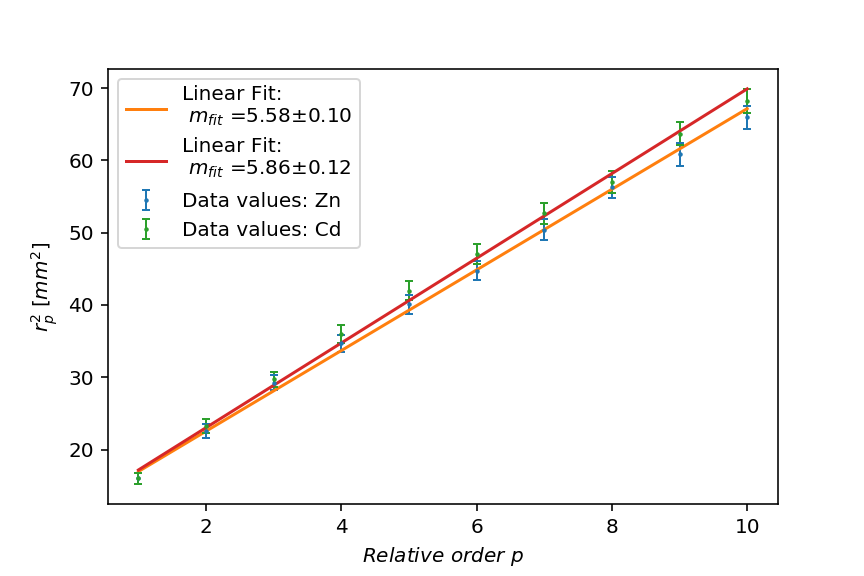
\includegraphics[width=1\textwidth]{Plots/Lambda_Cd_Zn.png}
\caption{Visualisation of the taken values for zinc and cadmium lamps red spectral line. The gradient of the linear fit will be used to calculate its wavelength.}
\label{fig: lambda cd zn }
\end{figure}

The values are fitted with the linear equation given in \autoref{eq:lambda fit func}. The linear relation between the order and the $r_p^2$ is good represented. With \autoref{eq: lambda dlambda} the following wavelengths are calculated.

\begin{equation}
\lambda_0= \frac{m_{fit}d}{f^2} \;,\quad \Delta\lambda_0=\sqrt{ \left(\frac{\Delta m_{fit}d}{f^2}\right)^2 +\left(\frac{m_{fit}\Delta d}{f^2}\right)^2 +\left(\frac{m_{fit}d\Delta f}{f^3}\right)^2 }
\label{eq: lambda dlambda}
\end{equation}

\begin{table}[H]
\centering
\begin{tabular}{c|c|c|c}
Lamp & Gradient $m_{fit}$ $[mm^2]$ & Wavelength $\lambda_0$ $[nm]$ & Literature $[nm]$ \\ \hline\hline
Zinc & $5.58 \pm 0.10$  & $935.69 \pm 35.89$ & $636.24$ \\ \hline
Cadminum & $5.86 \pm 0.12$  & $982.72 \pm 39.37$ & $643.85$
\end{tabular}
\caption{Measured gradients and calculated wavelengths for both lamp without the polarisation filter. The expected values are give in the script for this experiment, see \cite{wiki}}
\label{tab:lam 0}
\end{table}

\autoref{tab:lam 0} shows the calculated values. Our values are very different from the expected values. Nevertheless the wavelength of zinc is smaller than the one from cadmium, which was expected. It seems like there was a systematic error, that increased the our values by $300nm$ or additional $50\%$.


\subsection{Zeeman effect}
The following parts are always done with the cadmium lamp. To begin with we looked at the dispersion zone for a increasing magnetic field. The dispersion zone is defined as the relative position of maximum of the $\sigma^+$ light and the next orders $\sigma^-$. $1/2$ dispersion zone is reached if those two maxima are at the same position. The values $1/4$ and $3/4$ are given when the distance between the lights of each order is the same, meaning there are twice as many peak as in the case without magnetic field or $1/2$ dispersion zone. The difference for those cases is the magnetic field strength. The results are shown in \autoref{tab:dispersion zone}. The magnetic field is calculated with \autoref{eq:B fit} and \autoref{eq: B error}.

\begin{table}[H]
\centering
\begin{tabular}{c|c|c}
Dispersion zone & Current I $[A]$ & Mag. Field B $[mT]$ \\ \hline\hline
1/4 & $9 \pm 1$  & $194.08 \pm 19.53$  \\ \hline
1/2 & $18 \pm 1.5$  & $356.47 \pm 24.61$  \\ \hline
3/4 & $32 \pm 1$  & $542.18 \pm 9.76$ 
\end{tabular}
\caption{ Current values and magnetic fields for different dispersion zones. }
\label{tab:dispersion zone}
\end{table}

The same procedure as before is now applied for the case with $\lambda/4$ wave plate and polarisation filter at $1/4$ dispersion zone. By changing the polarisation filter we were able to observe the transition from $\sigma^+$ and $\sigma^-$ polarised light. The position of the maxima shifted not continuously by moving to another location. It was more like one faded away while the other ring slowly appeared.

From theory we already know that the $\sigma^+$ light has the higher energy and therefore the shorter wavelength: $\lambda_{\sigma^+} < \lambda_{\sigma^-}$. This will help us to determine which wavelength corresponds to which polarisation.

\begin{table}[H]
\centering
\begin{tabular}{c|c|c}
Polarisation & Gradient $m_{fit}$ $[mm^2]$ & Wavelength $[nm]$ \\ \hline\hline
$\sigma^+$ & $6.35 \pm 0.14$  & $1065.59 \pm 43.37$  \\ \hline
$\sigma^-$ & $6.47 \pm 0.20$  & $1085.33 \pm 49.86$  
\end{tabular}
\caption{Calculated wavelengths for the linear fit which is shown in \autoref{fig: lambda sigma pm}.}
\label{tab: lam sigmas}
\end{table}

Again the wavelengths not around the expected value of $643.85nm$, even differing form the results in \autoref{tab:lam 0} with $\lambda_0 = 982.72\pm39.37 nm$. But the relative shift of the Zeeman effect is nicely illustrated.

A comparison between energy difference of the wavelengths and the expected difference due to the magnetic field is shown below. The magnetic field for $1/4$ dispersion zone is used.

\begin{align}
\delta E_\lambda &= hc\cdot k := hc\left(\frac{1}{\lambda_1}- \frac{1}{\lambda_2}\right) = 0.0217 eV \\
\delta E_B &= 2\mu_B B = \frac{\hbar}{m_e}B = 0.0000225 eV 
\label{eq: 10^3 faktor}
\end{align}

The wavelength differences are larger than expected. Due to their large error this is a possibility. For wavelengths closer to each other the energy difference could become the expected one.

\begin{figure}[H]
\centering
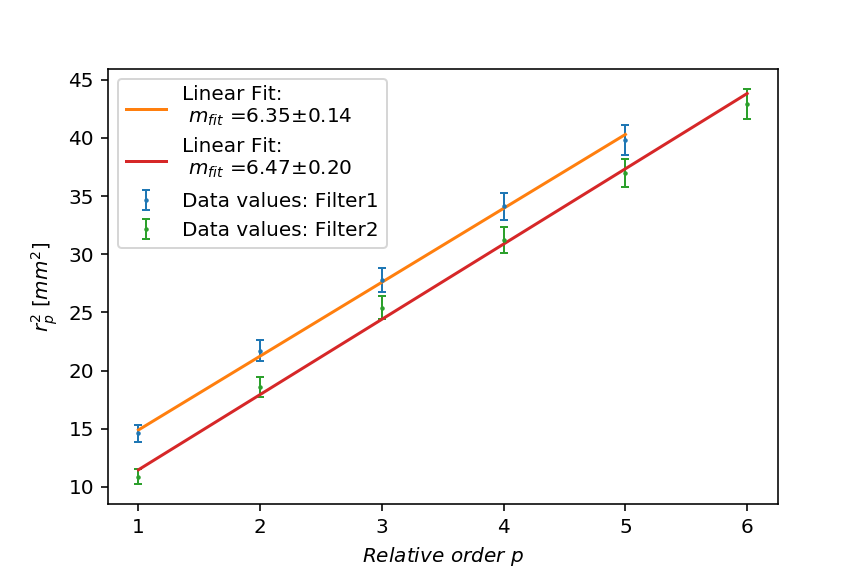
\includegraphics[width=1\textwidth]{Plots/Both_Filters.png}
\caption{Determination of the wavelength for two different positions of the polarisation filter. The values were taken for the highest intensity of the maxima of each polarisation.}
\label{fig: lambda sigma pm}
\end{figure}


\subsection{Resolving Capacity}
The expected resolving capacity for the Fabry-Pérot Interferometer was given in \autoref{eq:resolving cap}. This will be compared to the values taken when the line started to split up. For this only three orders were clearly visible. The current was $6\pm 0.5 A \overset{\land}{=} 134.19 \pm 10.19 mT$. 
With \autoref{eq: resolving capacity herleitung} the measured one is calculated.

In these equations $\delta$ incicates the difference, while $\Delta$ is describing the error on the value. The value for $\lambda_0$ will be given by the entry for cadmium from \autoref{tab:lam 0} with $\lambda_0 = 982.72\pm39.37 nm$.

\begin{align}
\delta E= hc \cdot k\ =\ hc \frac{\lambda_1-\lambda_2}{\lambda_1\lambda_2}\ \approx\ hc\frac{\delta \lambda}{\lambda_0^2}\ \overset{!}{=}\ 2\mu_B B 
\label{eq: delta E gleich}
\\
\frac{\lambda_0}{\delta \lambda} = \frac{hc}{2\mu_B B \lambda_0} \;,\quad \Delta \frac{\lambda_0}{\delta \lambda} = \frac{hc}{2\mu_B B \lambda_0} \cdot \sqrt{\left(\frac{\Delta \lambda_0}{\lambda_0}\right)^2 + \left(\frac{\Delta B}{B}\right)^2}
\label{eq: resolving capacity herleitung}
\end{align}

\begin{table}[H]
\centering
\begin{tabular}{c|c}
&$\lambda_0/\delta\lambda$ $[10^4]$\\ \hline\hline
Theory & $960.6 \pm 38.5$    \\ \hline
Measured & $8.1 \pm 0.7$  
\end{tabular}
\caption{Results from the calculations of the resolving capacity.}
\label{tab: res cap results}
\end{table}

The calculated values for the resolving capacity are shown in \ref{tab: res cap results}. Expected was a lower value than given by theory, but the difference is extreme. Only $1\%$ of the best resolution seems to be very bad. This could already explain the discrepancy in the wavelengths, see \autoref{tab:lam 0}.


\subsection{Electrons specific charge}
The specific charge of the electron $e/m_e$ is now calculate by the definition of $\mu_b = \hbar e/2m_e$ . The values for the Zeeman effect will be used, see \autoref{tab: lam sigmas}. \autoref{eq: spec charge} follows by \autoref{eq: delta E gleich}.

\begin{equation}
\frac{e}{m_e} = \frac{2\pi c}{B} \cdot k \;,\quad \Delta \frac{e}{m_e} = \frac{2\pi c}{B} \sqrt{\left(\frac{\Delta B}{B}\cdot k \right)^2 + \left(\frac{\Delta\lambda_1}{\lambda_1^2}\right)^2 + \left(\frac{\Delta\lambda_2}{\lambda_2^2}\right)^2 }
\label{eq: spec charge}
\end{equation}

\begin{table}[H]
\centering
\begin{tabular}{c|c}
&$e/m_e$ $[10^{11} C/kg]$\\ \hline\hline
Theory & $ 1.7588 $    \\ \hline
Measured & $1.6566 \cdot 10^3 \pm 1946.61 \cdot 10^3 $  
\end{tabular}
\caption{Results from the calculations of the specific charge.}
\label{tab: e/me results}
\end{table}

Again the result differs by a factor of $10^3$ and the large error shows that something didn't work as expected. The large errors on the both wavelengths for $\sigma^+$ and $\sigma^-$ polarised light are causing the large derivation. The value itself could be nicely fitting if the magnetic field unit is $[T]$ instead of $[mT]$, but such a strong magnetic field seems very wrong.


\newpage
\section{Error discussion and Conclusion}
The large error bars are caused by the large distances $r_p$ and the linear fit. We assumed an error of $0.1mm$ on the distances due to the thickness of the rings. By measuring relative to the center the distances could have been smaller and thereby a better fit would have been possible, but this shouldn't affect the measured value, only the error. Due to the large errors and the propagation of uncertainty the determination of the specific charge ended in an error 2000 times larger than the value itself.

The difference of the factor $10^3$ is still untraceable. Calculating \autoref{eq: 10^3 faktor} in SI units this value should be right. The small offset on the hysteresis calibration, due to the hall probes are always measuring a small magnetic field. Those fluctuations don't explain the large difference for the shown values. Although the magnetic field should be nearly the same in between the coils, the later position of the lamp relative to the location we measured the magnetic field, could cause some variation.

Our small resolving capacity reinforces the assumption that the we couldn't measure the wavelengths as precise as wanted to. It seems like the wavelength is also depending on the settings we used to display the on the monitor. Before taking the values of the Zeeman shift we had to recalibrate the camera setting to visualise the rings. This could explain why $\lambda_0$ is not between the wavelengths of both circular polarised lights. See Appendix for \autoref{fig: not used}, which was taken to calculate the resolving capacity for another different setting. Again the wavelengths are different for the same spectral line are changing the camera settings.

Maybe also the numbering of our maxima was wrong, but we didn't see any other, which could justify to skip an order. This would reduce the overall wavelengths. External light sources should not have affected the experiment, because the rings were red.
\\ \\
In the end the Zeeman shift was recorded but the calculations failed somehow. We were not able to determine the systematic error which causes the wavelengths to differ from the expected values. The calibration of the magnetic field showed a good hysteresis, but some how the energy differences are differing by $10^3$. 

We didn't checked if the beam path was optimal to create the best possible interference. By checking the focal planes and the function of $\lambda/4$ plate and polarisation filter, error sources could be excluded to find the real reason.


\newpage
\section{Appendix}
\begin{figure}[H]
\centering
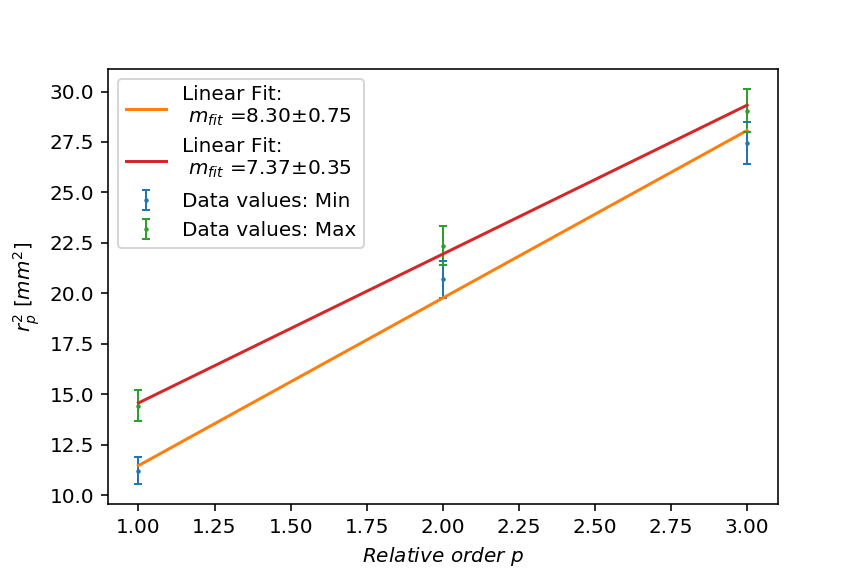
\includegraphics[width=1\textwidth]{Plots/Res_Cap.png}
\caption{Additional attempt to calculate the resolving capacity of the FPI. It was not used due to the extremely differing wavelengths from the shown gradients. The values are bad due to an insufficient amount of data values for the fit.}
\label{fig: not used}
\end{figure}


\newpage
\begin{thebibliography}{}
\bibitem[Dem3]{dem3} Demtröder Experimentalphysik 3: Atome, Moleküle und Festkörper, Springer

\bibitem[F Wiki]{wiki} \begin{verbatim}
http://wiki-fp.physik.uni-mainz.de/index.php/
1_Zeeman_effect
\end{verbatim} 


\end{thebibliography}
\end{document}

